\documentclass[a4paper]{article}
\usepackage[a4paper,margin=0mm]{geometry}
\usepackage{fontspec}
\usepackage{unicode-math}
\usepackage{tikz}
\usepackage[table]{xcolor}
\usepackage[absolute]{textpos}
\usepackage{enumitem}
\usepackage{array}
\usepackage{multirow}

\setmainfont{Libertinus Serif}
\setsansfont{Libertinus Sans}
\setmathfont{Libertinus Math}
\newfontfamily\trackedsans{Libertinus Sans}[LetterSpace=8.0]

\definecolor{accent}{HTML}{602785}
\definecolor{badge}{HTML}{B8A0C8}
\definecolor{ink}{HTML}{2A2E30}

\setlength{\TPHorizModule}{1mm}
\setlength{\TPVertModule}{1mm}
\setlength{\parindent}{0pt}
\pagestyle{empty}

\newcommand{\LCOL}{16mm}
\newcommand{\RCOL}{111mm}
\newcommand{\COLW}{83mm}

\newcommand{\topicheader}[2]{%
\begin{textblock*}{194mm}(16mm,10mm)
\begin{tikzpicture}
\node[fill=accent,text=white,font=\sffamily\bfseries\fontsize{13}{13}\selectfont,
      minimum width=9mm,minimum height=9mm,inner sep=0pt] at (4.5mm,-4.5mm) {#1};
\node[font=\sffamily\bfseries\fontsize{15}{16}\selectfont,text=ink,anchor=west] at (12mm,-4.5mm) {#2};
\end{tikzpicture}
\end{textblock*}
\begin{textblock*}{194mm}(16mm,22.5mm)

\begin{tikzpicture}
\fill[accent] (0,0) rectangle (194mm,0.5mm);
\end{tikzpicture}
\end{textblock*}
}

\newcommand{\pagefooter}[1]{%
\begin{textblock*}{194mm}(8mm,286.41mm)
  
\begin{tikzpicture}
    \fill[accent] (0,0) rectangle (194mm,0.6mm);
  \end{tikzpicture}
\end{textblock*}
\begin{textblock*}{63.59mm}(8mm,288.27mm)
  {\sffamily\bfseries\color{accent}\fontsize{13}{16}\selectfont SAT 1200+}
\end{textblock*}
\begin{textblock*}{10mm}(188mm,288.27mm)
  \centering{\sffamily\color{accent}\fontsize{14}{16}\selectfont #1}
\end{textblock*}
}

\newcommand{\colrule}[2]{%
\begin{textblock*}{1mm}(105mm,#1mm)
\begin{tikzpicture}
\draw[black!65,line width=0.5pt] (0,0) -- (0,#2mm);
\end{tikzpicture}
\end{textblock*}
}

\newcommand{\setkicker}[2]{%
{\sffamily\bfseries\fontsize{12}{14}\selectfont #1.}\ {\itshape\fontsize{11}{14}\selectfont\color{black!75} #2}\par\vspace{2mm}%
}

\setlength{\fboxsep}{1.4pt}
\setlength{\fboxrule}{0.5pt}
\newcommand{\pnum}[1]{\fcolorbox{ink}{white}{\sffamily\bfseries\fontsize{8}{8}\selectfont #1}~}

\newcommand{\qrbox}[1]{%
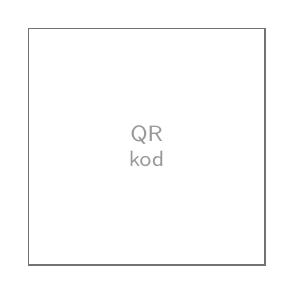
\begin{tikzpicture}
\draw[black!55,line width=0.6pt] (0,0) rectangle (30mm,30mm);
\node[black!40,font=\sffamily\fontsize{8}{9}\selectfont,align=center] at (15mm,15mm) {QR\\kod};
\end{tikzpicture}\\[1.5mm]
{\sffamily\fontsize{9}{11}\selectfont\color{black!70} #1}%
}

\arrayrulecolor{accent}
\setlength{\arrayrulewidth}{0.7pt}
\renewcommand{\arraystretch}{1.35}
\newcommand{\anstitle}[1]{{\sffamily\bfseries\color{accent}\fontsize{11}{13}\selectfont #1}\\[1.3mm]}

\begin{document}

% ================= PAGE 1: Set 1 | Set 2 =================
\topicheader{8}{Eksponensial o'sish va kamayish}
\pagefooter{1}
\colrule{32}{238}
\mbox{}%

\begin{textblock*}{\COLW}(\LCOL,32mm)
{\fontsize{11}{14}\selectfont
\setkicker{1-to'plam}{Jadval chiziqlimi yoki eksponensialmi? Qoidasini ($y=\ldots$) yozing.}

\noindent\pnum{1} $y = 5,\ 10,\ 20,\ 40$\par\vspace{16mm}
\noindent\pnum{2} $y = 3,\ 7,\ 11,\ 15$\par\vspace{16mm}
\noindent\pnum{3} $y = 100,\ 90,\ 81,\ 72.9$\par\vspace{16mm}
\noindent\pnum{4} $y = 50,\ 45,\ 40,\ 35$\par\vspace{16mm}
\noindent\pnum{5} $y = 2,\ 6,\ 18,\ 54$\par\vspace{16mm}
\noindent\pnum{6} $y = 10,\ 12.5,\ 15,\ 17.5$
}
\end{textblock*}

\begin{textblock*}{\COLW}(\RCOL,32mm)
{\fontsize{11}{14}\selectfont
\setkicker{2-to'plam}{O'sish: tenglama tuzing, so'ng hisoblang.}

\noindent\pnum{1} A town's population is 200 and grows 5\% per year. Find the population after 4 years.\par\vspace{11mm}
\noindent\pnum{2} An investment of \$1000 grows 6\% per year. Find its value after 3 years.\par\vspace{11mm}
\noindent\pnum{3} A bacteria culture starts at 50 and doubles every hour. Find the count after 5 hours.\par\vspace{11mm}
\noindent\pnum{4} A city's population is 8000 and grows 3\% per year. Find the population after 2 years.\par\vspace{11mm}
\noindent\pnum{5} An item costs \$20 and its price increases 10\% per year. Find the price after 3 years.\par\vspace{11mm}
\noindent\pnum{6} A quantity starts at 12 and grows by a factor of 1.5 each step. Find its value after 4 steps.
}
\end{textblock*}

\clearpage

% ================= PAGE 2: Set 3 | Set 4 =================
\topicheader{8}{Eksponensial o'sish va kamayish}
\pagefooter{2}
\colrule{32}{238}
\mbox{}%

\begin{textblock*}{\COLW}(\LCOL,32mm)
{\fontsize{11}{14}\selectfont
\setkicker{3-to'plam}{Kamayish: tenglama tuzing, so'ng hisoblang.}

\noindent\pnum{1} A car worth \$15000 depreciates 12\% per year. Find its value after 3 years.\par\vspace{11mm}
\noindent\pnum{2} A 200 g sample decreases 8\% per year. Find the amount after 2 years.\par\vspace{11mm}
\noindent\pnum{3} A population of 5000 declines 4\% per year. Find the population after 5 years.\par\vspace{11mm}
\noindent\pnum{4} 100 mg of medication decreases 25\% every hour. Find the amount after 3 hours.\par\vspace{11mm}
\noindent\pnum{5} An 800 L tank loses 10\% of its water each day. Find the amount after 2 days.\par\vspace{11mm}
\noindent\pnum{6} A \$2000 value decreases by a factor of 0.8 each year. Find the value after 3 years.
}
\end{textblock*}

\begin{textblock*}{\COLW}(\RCOL,32mm)
{\fontsize{11}{14}\selectfont
\setkicker{4-to'plam}{Avval chiziqli/eksponensialligini aniqlang, so'ng hisoblang.}

\noindent\pnum{1} A plant grows 3 cm every week, starting at 10 cm. Height after 6 weeks?\par\vspace{11mm}
\noindent\pnum{2} A savings account earns 4\% interest per year, starting at \$500. Value after 3 years?\par\vspace{11mm}
\noindent\pnum{3} A phone loses 15\% of its charge every hour, starting at 100\%. Charge after 2 hours?\par\vspace{11mm}
\noindent\pnum{4} A pool drains at a constant rate of 50 liters per minute, starting with 2000 liters. Amount after 10 minutes?\par\vspace{9mm}
\noindent\pnum{5} Bacteria triple every day, starting with 4. Count after 4 days?\par\vspace{11mm}
\noindent\pnum{6} A runner's distance increases by 2 miles every day, starting at 1 mile. Distance after 5 days?
}
\end{textblock*}

\clearpage

% ================= PAGE 3: Set 5 | Set 6 (spot the error) =================
\topicheader{8}{Eksponensial o'sish va kamayish}
\pagefooter{3}
\colrule{32}{238}
\mbox{}%

\begin{textblock*}{\COLW}(\LCOL,32mm)
{\fontsize{11}{14}\selectfont
\setkicker{5-to'plam}{Yarimparchalanish davri (half-life).}

\noindent\pnum{1} 160 g of a substance has a half-life of 4 years. How much remains after 12 years?\par\vspace{18mm}
\noindent\pnum{2} 500 mg of a drug has a half-life of 6 hours. How much remains after 18 hours?\par\vspace{18mm}
\noindent\pnum{3} 80 g of an isotope has a half-life of 10 days. How much remains after 30 days?\par\vspace{18mm}
\noindent\pnum{4} A population halves every 5 years, starting at 6400. Find the population after 20 years.\par\vspace{18mm}
\noindent\pnum{5} 1000 bacteria die off such that the count halves every 3 hours. Find the count after 9 hours.
}
\end{textblock*}

\begin{textblock*}{\COLW}(\RCOL,32mm)
{\fontsize{11}{14}\selectfont
\setkicker{6-to'plam}{Xatoni toping -- buzilgan qadamni ayting, to'g'ri javobni bering.}

\noindent\pnum{1} A city grows 7\% per year, starting at 10000. Find the population after 2 years --\\
\hspace*{7mm}\textit{``$10000\times(1.7)^2=28900$.''}\\[2mm]
\hspace*{7mm}Xato va to'g'ri javob: \makebox[50mm]{\dotfill}\\[6mm]

\noindent\pnum{2} A sample decreases 20\% per year, starting at 500. Find the amount after 2 years --\\
\hspace*{7mm}\textit{``$500\times(1+0.2)^2=720$.''}\\[2mm]
\hspace*{7mm}Xato va to'g'ri javob: \makebox[50mm]{\dotfill}\\[6mm]

\noindent\pnum{3} A table shows $y=2,4,8,16$ for $x=0,1,2,3$ --\\
\hspace*{7mm}\textit{``This is linear with common difference 2, so $y=2+2x$.''}\\[2mm]
\hspace*{7mm}Xato va to'g'ri javob: \makebox[50mm]{\dotfill}\\[6mm]

\noindent\pnum{4} A car depreciates by \$1500/year, starting at \$20000 --\\
\hspace*{7mm}\textit{``This is exponential: $y=20000\times(1-0.075)^t$.''}\\[2mm]
\hspace*{7mm}Xato va to'g'ri javob: \makebox[50mm]{\dotfill}\\[6mm]

\noindent\pnum{5} Amount remaining after 3 half-lives, starting at 240 g --\\
\hspace*{7mm}\textit{``$240-3\times\frac12\times240=240-360=-120$.''}\\[2mm]
\hspace*{7mm}Xato va to'g'ri javob: \makebox[50mm]{\dotfill}
}
\end{textblock*}

\clearpage

% ================= PAGE 4: Set 7 (bonus, work backward) =================
\topicheader{8}{Eksponensial o'sish va kamayish}
\pagefooter{4}
\colrule{32}{238}
\mbox{}%

\begin{textblock*}{\COLW}(\LCOL,32mm)
{\fontsize{11}{14}\selectfont
\setkicker{7-to'plam}{Bonus / qiyin -- teskari masala: berilgan natijadan parametrni toping.}

\noindent\pnum{1} A population grows from 200 to 242 in 2 years at a constant annual percent rate. Find the rate.\par\vspace{20mm}
\noindent\pnum{2} A substance decays to $\frac14$ of its original amount after 10 days. Find its half-life.\par\vspace{20mm}
\noindent\pnum{3} An investment grows from \$1000 to \$1331 in 3 years at a constant annual rate. Find the rate.\par\vspace{20mm}
\noindent\pnum{4} A car worth \$25000 depreciates to \$20000 after 1 year at a constant percent rate. Find the rate, then predict the value after a total of 2 years.\par\vspace{16mm}
\noindent\pnum{5} A quantity grows from 3 to 48 over 4 equal steps. Is this linear or exponential? Find the rule.
}
\end{textblock*}

\clearpage

% ================= PAGE 5: Javoblar part 1 -- Sets 1-4 =================
\topicheader{8}{Eksponensial o'sish va kamayish}
\pagefooter{5}
\mbox{}%

\begin{textblock*}{194mm}(16mm,30mm)
{\bfseries\itshape\color{accent}\fontsize{19}{21}\selectfont\centering Javoblar\par}
\end{textblock*}

\begin{textblock*}{194mm}(16mm,46mm)
{\fontsize{10}{12.5}\selectfont
\centering
\renewcommand{\arraystretch}{1.3}
\begin{tabular}{|>{\centering\arraybackslash}p{24mm}|>{\centering\arraybackslash}p{9mm}|p{145mm}|}
\hline
\rowcolor{badge!55}\textbf{To'plam} & \textbf{\#} & \textbf{Javob}\\
\hline
\multirow{6}{24mm}{\centering 1-to'plam} & 1 & Exponential, $y=5\times2^x$\\\cline{2-3}
 & 2 & Linear, $y=3+4x$\\\cline{2-3}
 & 3 & Exponential, $y=100\times0.9^x$\\\cline{2-3}
 & 4 & Linear, $y=50-5x$\\\cline{2-3}
 & 5 & Exponential, $y=2\times3^x$\\\cline{2-3}
 & 6 & Linear, $y=10+2.5x$\\\hline
\multirow{6}{24mm}{\centering 2-to'plam} & 1 & $\approx243$\\\cline{2-3}
 & 2 & $\approx\$1191.02$\\\cline{2-3}
 & 3 & $1600$\\\cline{2-3}
 & 4 & $\approx8487$\\\cline{2-3}
 & 5 & $\approx\$26.62$\\\cline{2-3}
 & 6 & $60.75$\\\hline
\multirow{6}{24mm}{\centering 3-to'plam} & 1 & $\approx\$10222.08$\\\cline{2-3}
 & 2 & $\approx169.28$ g\\\cline{2-3}
 & 3 & $\approx4077$\\\cline{2-3}
 & 4 & $\approx42.19$ mg\\\cline{2-3}
 & 5 & $648$ L\\\cline{2-3}
 & 6 & $\$1024$\\\hline
\multirow{6}{24mm}{\centering 4-to'plam} & 1 & Linear, $28$ cm\\\cline{2-3}
 & 2 & Exponential, $\approx\$562.43$\\\cline{2-3}
 & 3 & Exponential, $\approx72.25\%$\\\cline{2-3}
 & 4 & Linear, $1500$ L\\\cline{2-3}
 & 5 & Exponential, $324$\\\cline{2-3}
 & 6 & Linear, $11$ miles\\\hline
\end{tabular}
}
\end{textblock*}

\clearpage

% ================= PAGE 6: Javoblar part 2 -- Sets 5-7 + QR =================
\topicheader{8}{Eksponensial o'sish va kamayish}
\pagefooter{6}
\mbox{}%

\begin{textblock*}{194mm}(16mm,32mm)
{\fontsize{10}{12.5}\selectfont
\centering
\renewcommand{\arraystretch}{1.3}
\begin{tabular}{|>{\centering\arraybackslash}p{24mm}|>{\centering\arraybackslash}p{9mm}|p{145mm}|}
\hline
\rowcolor{badge!55}\textbf{To'plam} & \textbf{\#} & \textbf{Javob}\\
\hline
\multirow{5}{24mm}{\centering 5-to'plam} & 1 & $20$ g\\\cline{2-3}
 & 2 & $62.5$ mg\\\cline{2-3}
 & 3 & $10$ g\\\cline{2-3}
 & 4 & $400$\\\cline{2-3}
 & 5 & $125$\\\hline
\multirow{5}{24mm}{\centering 6-to'plam} & 1 & Error -- $7\%$ treated as $1.7$ instead of $1.07$. To'g'ri: $10000\times1.07^2\approx11449$.\\\cline{2-3}
 & 2 & Error -- used $(1+r)$ for a decaying quantity instead of $(1-r)$. To'g'ri: $500\times0.8^2=320$.\\\cline{2-3}
 & 3 & Error -- differences $2,4,8$ are not constant; ratios $2,2,2$ are constant, so it's exponential: $y=2\times2^x$.\\\cline{2-3}
 & 4 & Error -- a constant dollar amount per year is linear, not exponential. To'g'ri: $y=20000-1500t$.\\\cline{2-3}
 & 5 & Error -- treated repeated halving as subtraction instead of multiplication. To'g'ri: $240\times(\frac12)^3=30$ g.\\\hline
\multirow{5}{24mm}{\centering 7-to'plam} & 1 & $r=10\%$\\\cline{2-3}
 & 2 & $h=5$ days\\\cline{2-3}
 & 3 & $r=10\%$\\\cline{2-3}
 & 4 & $r=20\%$; after 2 years, $\$16000$\\\cline{2-3}
 & 5 & Exponential, $y=3\times2^x$\\\hline
\end{tabular}
}
\end{textblock*}

\begin{textblock*}{194mm}(16mm,220mm)
\centering
{\sffamily\fontsize{9.5}{11.5}\selectfont\color{black!70} Video yechimlar va qo'shimcha testlar uchun quyidagi QR kodlarni skanerlang:}\\[4mm]
\begin{minipage}[t]{32mm}\centering\qrbox{YouTube}\end{minipage}%
\hspace{16mm}%
\begin{minipage}[t]{32mm}\centering\qrbox{Telegram}\end{minipage}
\end{textblock*}

\end{document}
